\section{Image charge}
\subsection{Screened interaction and image charge problem}

\begin{exercise}
We consider a point charge $q$ (we use atomic units so $q$ is measured in units of the elementary charge $e$) located a distance $z$ outside a semi-infinite metal surface. Argue that the potential energy of the point charge is given by
\begin{equation}
    V_{img}(r) = - \frac{q^2}{4z}
\end{equation}
\end{exercise}

\begin{solution}
The conductor will respond to the point charge by screening, which will create an electric field opposing it, so that there is no netto field inside the conductor. This electric field is not very easy to compute, however this problem is the same as another problem. To see this we need to use that the tangential component of the electric field to the surface is continuous across the surface, however since there is no E-field inside the conductor the field lines must point perpendicularly into the surface.


\begin{figure}[!ht]
    \centering
    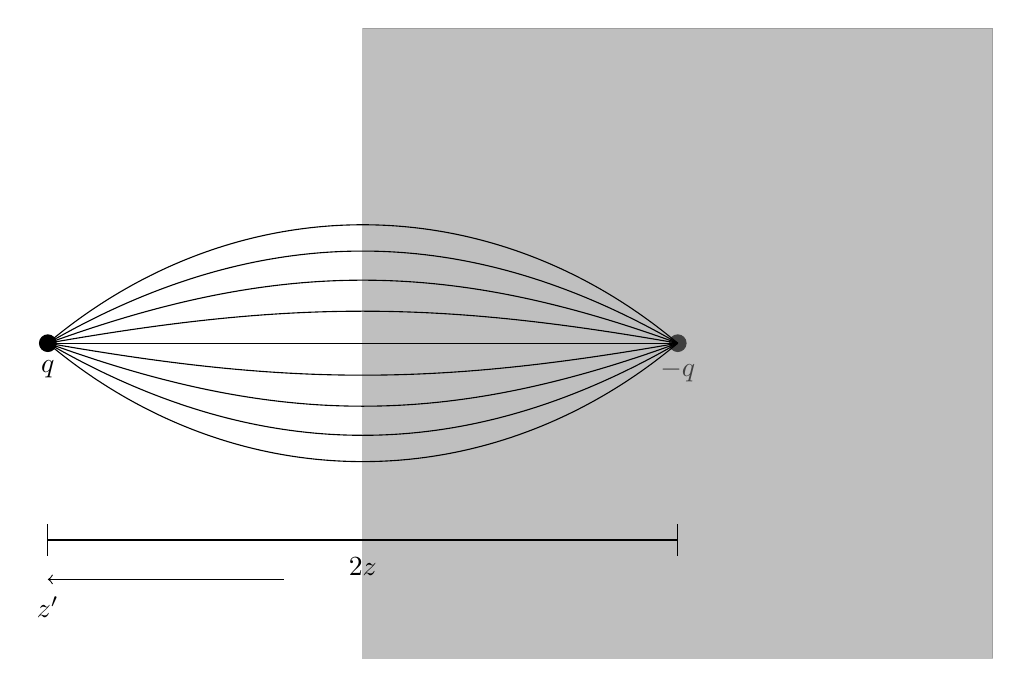
\begin{tikzpicture}
    \filldraw (0,0) circle (3pt);
    \draw (0,-0.1) node[below] {$q$};
    \filldraw (8,0) circle (3pt);
    \draw (8,-0.1) node[below] {$-q$};
    \draw [fill=gray,gray,opacity=0.5] (4,-4) rectangle (12,4); 
    \draw[-] (0,0) to (8,0);
    \draw[-] (0,0) to [out = 40, in=140] (8,0);
    \draw[-] (0,0) to [out = 30, in=150] (8,0);
    \draw[-] (0,0) to [out = 20, in=160] (8,0);
    \draw[-] (0,0) to [out = 10, in=170] (8,0);
    \draw[-] (0,0) to [out = -40, in=-140] (8,0);
    \draw[-] (0,0) to [out = -30, in=-150] (8,0);
    \draw[-] (0,0) to [out = -20, in=-160] (8,0);
    \draw[-] (0,0) to [out = -10, in=-170] (8,0);
    
    \draw[-] (0,-2.5) to (8,-2.5);
    \draw[-] (0,-2.7) to (0,-2.3);
    \draw[-] (8,-2.7) to (8,-2.3);
    \draw (4,-2.6) node[below] {$2z$};
    
    \draw[<-] (0,-3) -- (3,-3);
    \draw (0,-3.1) node[below] {$z'$};
    
    
    \end{tikzpicture}
    \caption{Illustration of the problem, where we instead solve the equivalent problem of the image charge. The conductor above should be imagined to be infinite. The drawn lines illustrates the E-field which are the same regardless if we are looking at the problem with two charges, or the one with one charge and a conductor}
    \label{fig:ImageCharge}
\end{figure}
The force between the two particles in atomic units is given by the Coulombs force
\begin{equation}
    F = - \frac{q^2}{(2z)^2}
\end{equation}
Which means that the potential energy of the point charge is given by
\begin{equation}
    V_{img} = \int_{\infty}^z F \mathrm{d}z' = -\int_{\infty}^z \frac{q^2}{4z} \mathrm{d}z' = -\frac{q^2}{4z}
\end{equation}
Where $z$ is chosen as the upper limit as this is the distance between the point charge and the conductor.
\end{solution}


\begin{exercise}
Argue that the potential at point $r'$ due to the charge density induced in the surface bu a unit charge ($q=e$) point charge at position $r$ is given by
\begin{equation}
    \Delta W_{img}(r,r') = -\frac{1}{2} [(x-x')^2 + (y-y')^2 + (z+z')^2]^{-1/2}
\end{equation}
Note that $\Delta W_{img}(r,r) = V_{img}(r)$ as it should.
\end{exercise}
\begin{solution}

\begin{figure}[!ht]
    \centering
    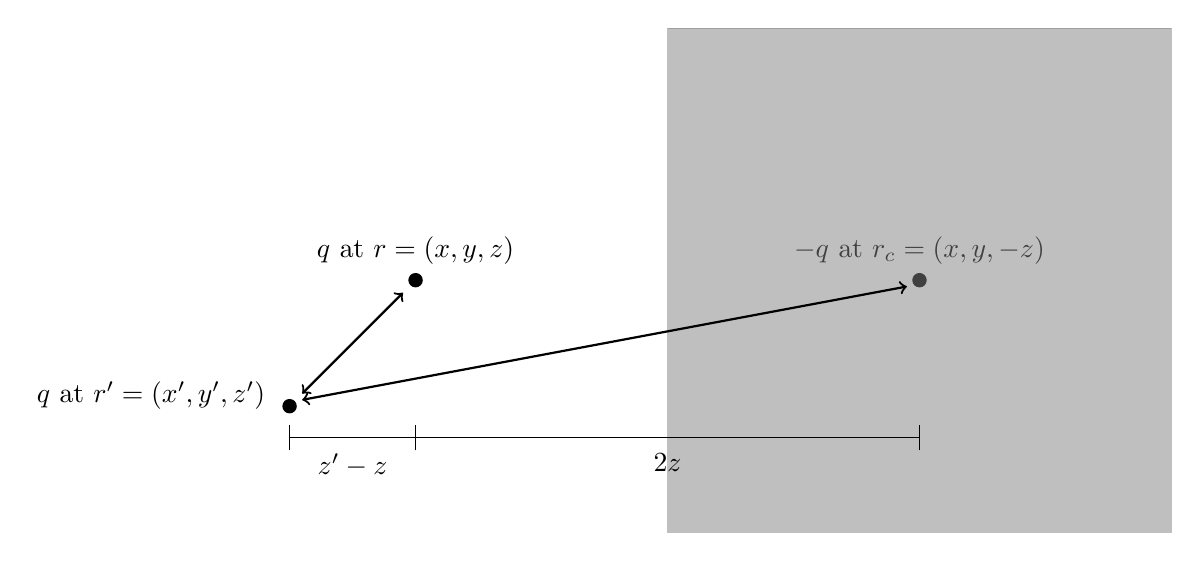
\begin{tikzpicture}[scale=0.8]
    
    
    %Circles
    \filldraw (0,0) circle (3pt);
    \draw (0,0.1) node[above] {$q$ at $r=(x,y,z)$};
    \filldraw (8,0) circle (3pt);
    \draw (8,0.1) node[above] {$-q$ at $r_c = (x,y,-z)$};
    \filldraw (-2,-2) circle (3pt);
    \draw (-4.2,-2.2) node[above] {$q$ at $r'=(x',y',z')$};
    
    %Conductor
    \draw [fill=gray,gray,opacity=0.5] (4,-4) rectangle (12,4); 
   
   % Length scales
    \draw[-] (-2,-2.5) to (0,-2.5);
    \draw[-] (-2,-2.7) to (-2,-2.3);
    \draw[-] (0,-2.7) to (0,-2.3);
    \draw (-1,-2.6) node[below] {$z'-z$};
    
    \draw[-] (0,-2.5) to (8,-2.5);
    \draw[-] (0,-2.7) to (0,-2.3);
    \draw[-] (8,-2.7) to (8,-2.3);
    \draw (4,-2.6) node[below] {$2z$};
    
    %\draw[<-] (0,-3) -- (3,-3);
    %\draw (0,-3.1) node[below] {$z'$};
    %Arrows
    \draw[<->,thick] (-1.8,-1.8) to (-0.2,-0.2);
    \draw[<->,thick] (-1.8,-1.9) to (7.8,-0.1);
    \end{tikzpicture}
    \caption{The problem, now with an extra charge at $r'$}
    \label{fig:ImageCharge2}
\end{figure}
It is straight forward to show by following the same approach as above. There are two contributions for the charge at r', from the charge at r. One direct potential given by
\begin{equation}
    v_{direct} = \frac{q^2}{\sqrt{(x'-x)^2 + (y'-y)^2 + (z'-z)^2}}
\end{equation}
And one from the image charge induced by the charge at r given by
\begin{equation}
\begin{split}\label{eq:806}
    v_{image} = \frac{-q^2}{\sqrt{(x'-x)^2 + (y'-y)^2 + (z'-z +2z)^2}} \\ = \frac{-q^2}{\sqrt{(x'-x)^2 + (y'-y)^2 + (z'+z)^2}}
    \end{split}
\end{equation}
Where $v_{image}$ is exactly $\Delta W_{img}$ as defined in the problem. 
\end{solution}

\begin{exercise}
Show, using the well known relation between the dielectric function and the density response function, that the screened potential induced by the metal surface is given by
\begin{equation}
    \Delta W(r,r') = \int \int v(r,r_1)\chi(r_1,r_2)v(r_2,r')\mathrm{d}r_1\mathrm{d}r_2
\end{equation}
where 
\begin{equation}\label{eq:image_SI}
    W(r,r') = \int \epsilon^{-1}(r,r'')v(r',r)\mathrm{d}r'' \quad \mathrm{and} \quad \Delta W(r,r') = W(r,r') - v(r,r')
\end{equation}
\textbf{NB! Note that the index on the potential differs from the notes}.
\end{exercise}
\begin{solution}
The "well known" relation between the density response function and the dielectric function is given by
\begin{equation}
    \epsilon^{-1}(r,r'') = \delta(r-r'') + \int \dfrac{1}{\abs{r-r_1}}\chi(r_1,r'')\mathrm{d}r_1
\end{equation}
Inserting this in the definition of the induced potential, \eqref{eq:image_SI} right we get
\begin{equation}
    \Delta W(r,r') = \int\delta(r-r'')v(r'',r')\mathrm{d}r'' + \int\int \dfrac{1}{\abs{r-r_1}}\chi(r_1,r'')v(r'',r')\mathrm{d}r_1\mathrm{d}r'' - v(r,r')
\end{equation}
Evaluating the integral over the delta function and re-indexing $r'' \rightarrow r_2$, and rearranging we get 
\begin{equation}
    \Delta W(r,r') = v(r,r') - v(r,r') + \int \int \dfrac{1}{\abs{r-r_1}}\chi(r_1,r_2)v(r_2,r')\mathrm{d}r_1\mathrm{d}r_2
\end{equation}
Finally we recognise the Coulomb term as the potential $v(r,r_1)$ to get:
\begin{equation}
    \Delta W(r,r') =\int\int v(r,r_1)\chi(r_1,r_2)v(r_2,r')\mathrm{d}r_1\mathrm{d}r_2
\end{equation}
\end{solution}

\subsection{Energy levels from the COH-SEX approximation}
\begin{exercise}
Show that when the electron-electron interactions are included at the level of the COH-SEX approximation, the difference between the energy levels of the adsorbed and isolated molecules becomes approximately
\begin{align}
    \varepsilon_H - \varepsilon_H^{gas} &\approx \dfrac{1}{2}\mel{\Psi_H}{\Delta W}{\Psi_H} - (\abs{\Psi_H}^2,\Delta W,\abs{\Psi_{h}^2}) \\
    \varepsilon_L - \varepsilon_L^{gas} &\approx \dfrac{1}{2}\mel{\Psi_L}{\Delta W}{\Psi_L}
\end{align}
where $\Delta W(r,r') = W_{N}(r,r') - W_{F}(r,r')$ ($N$: near, $F$: far) is the difference between the screened interaction with and without the metal surface present and we have introduced the following shorthand notation for a double integral
\begin{equation}
    (f,A,g) = \int \int f(r)A(r,r')g(r') \mathrm{d}r\mathrm{d}r'
\end{equation}
\textbf{Note} that the exercise has the difference in the electron affinity defined as $\varepsilon_L-\varepsilon_H^{gas}$, which is a typo.
\end{exercise}
\begin{solution}
In the static version of the GW approximation, also called the COH-SEX approximation, the self energy takes the form of a non-local one-electron potential, given by:
\begin{equation}
    \Sigma(r,r') = \dfrac{1}{2}[W(r,r') - v(r,r')]\delta(r-r') - \rho(r,r')W(r,r')
\end{equation}
where $\rho$ is the one particle density matrix. 
Denoting the energies by a superscript "far" if the molecules are far away from the metal we may write the ionization potential of the system is given by $\varepsilon_H - \varepsilon_H^{gas}$ where $H$ refers to the HOMO. The QP energy levels and wave functions of the molecules fulfill the QP equation
\begin{equation}
    [H^{0} + \Sigma(\varepsilon_i^{QP})(r,r')]\ket{\Psi_i^{QP}} = \varepsilon_i^{QP}\ket{\Psi_i^{QP}}
\end{equation}
Hence we may find the difference in the ionisation energy of the system with and without the screened interaction by subtracting the QP equations for the two systems, which only differs by the self-energy term
\begin{equation}\label{eq:818}
    [H^{0} + \Sigma(\varepsilon_H)^{N} - H^{0} - \Sigma(\varepsilon_H^{F})]\ket{\Psi_H} = [\Sigma(\varepsilon_H^{N})-\Sigma(\varepsilon_H^{F})]\ket{\Psi_H} = (\varepsilon_H - \varepsilon_H^{gas})\ket{\Psi_H}
\end{equation}
\textbf{Note:} The wave functions may only be assumed to be the same as we are placing the molecule far enough away from the metal surface that we can assume that the orbitals do not overlap, which means the wave functions of the molecule are the same as if there were no metal surface. \\
Taking the expectation value involves a double integral over $r$ and $r'$ as the self-energy is non-local, hence the expectation value from of the Hamiltonian with the self energy may be stated as
\begin{equation}
    \int \mel{\Psi_{H}(r)}{\hat{H}_0\delta(r-r') +\Sigma(r,r')}{\Psi_H(r')}\mathrm{d}r'
\end{equation}
where we have explicitly treated the position dependence. Hence without the self-energy the inner product is defined in it usual form, which shows that $\hat{H}_0$ is diagonal in the $r$ basis. Evaluating equation \ref{eq:818} in the COH-SEX approximation yields:
\begin{equation}\label{eq:image_ionization}
    \begin{split}
        \varepsilon_H - \varepsilon_H^{gas} &\approx \int\dfrac{1}{2}\mel{\Psi_H}{[W_N(r,r')-v_N(r,r') - W_{F}(r,r') + v_{F}(r,r')]\delta(r-r')}{\Psi_H} \\
        &-\mel{\Psi_H}{\rho_{N}(r,r')W_{N}(r,r') -\rho_{F}(r,r')W_{F}(r,r')}{\Psi_H}\mathrm{d}r'
    \end{split}
\end{equation}
Evaluating the first expectation value, with $v_N = v_F$ reduces the expression to
\begin{equation}
    \int\mel{\Psi_H}{[\Delta W_{N}(r,r') - \Delta W_{F}(r,r')]\delta(r,r')}{\Psi_H}\mathrm{d}r' = \mel{\Psi_H}{\Delta W(r,r')}{\Psi_H}
\end{equation}
Analysing the second term in \eqref{eq:image_ionization} shows that we may similarly write it in terms of $\rho_{F}(r,r') = \ket{\Psi_H}\bra{\Psi_H} = \rho_{N}(r,r')$ and $\Delta W(r,r')$ to obtain
\begin{equation}
    \int \int \Psi_H^{*}(r)\Psi_H(r)\Psi_H^{*}(r')\Delta W(r,r') \Psi_H(r') \mathrm{d}r'\mathrm{d}r = \int \int \abs{\Psi_H}^2\Delta W(r,r') \abs{\Psi_H}^2\mathrm{d}r'\mathrm{d}r
\end{equation}
which is alternatively written as $(\abs{\Psi_H}^2,\Delta W(r,r'),\abs{\Psi_H}^2)$. Hence the ionisation energy from \eqref{eq:image_ionization} can be written as
\begin{equation}
    \varepsilon_H - \varepsilon_H^{gas} \approx \dfrac{1}{2}\mel{\Psi_H}{\Delta W}{\Psi_H} - \left(\abs{\Psi_H}^2,\Delta W,\abs{\Psi_H}^2\right)
\end{equation}
The electron affinity can be found from the LUMO state, following the same approach so that the equivalent of \eqref{eq:image_ionization} reads
\begin{equation}
    \varepsilon_L - \varepsilon_L^{gas} \approx \int \dfrac{1}{2}\mel{\Psi_L}{[W_{N}-W_{F}]\delta(r-r')}{\Psi_L} - \mel{\Psi_L}{\rho_N W_{N} - \rho_F W_{F}}{\Psi_L}\mathrm{d}r'
\end{equation}
Again the first term readily simplifies to 
\begin{equation}
    \int\mel{\Psi_L}{[W_{N}-W_{F}]\delta(r-r')}{\Psi_L} \mathrm{d}r'= \mel{\Psi_L}{\Delta W}{\Psi_L}
\end{equation}
The second term needs a more care full treatment as the density operator is given by $\rho_N(r,r') = \ket{\Psi_H(r)}\bra{\Psi_H(r')} = \rho_F(r,r')$, like before, because the only occupied state(s) contributing to the interacting density is the HOMO density. Consequently we have
\begin{equation}\label{eq:image_affinity}
    \int \mel{\Psi_L}{\rho_N W_{N} - \rho_F W_{F}}{\Psi_L}\mathrm{d}r' = \int\int \Psi^{*}_L(r)\Psi_H(r)\Psi^{*}_H(r')\Delta W(r,r')\Psi_L(r')\mathrm{d}r\mathrm{d}r'
\end{equation}
Assuming $\Delta W(r,r')$ to be approximately constant, across the molecule, \eqref{eq:image_affinity} reduces to the
\begin{equation}
    \Delta W \bra{\Psi_L}\ket{\Psi_H}\bra{\Psi_H}\ket{\Psi_L} = 0
\end{equation}
as $\Psi_L$ and $\Psi_H$ are orthogonal. Hence the electron affinity, in the COH-SEX approximation, takes the form
\begin{equation}
    \varepsilon_L - \varepsilon_L^{gas} \approx \mel{\Psi_L}{\Delta W}{\Psi_L}
\end{equation}
\end{solution}

\begin{exercise}
Use the classical model for the image charge potential $\Delta W$ and sketch how the HOMO and LUMO energy levels vary as function of the metal molecule separation.
\end{exercise}
\begin{solution}
Recalling that the quasi-particle energies $\varepsilon_H$ and $\varepsilon_L$ relates to the ionisation potential and electron affinity, respectively, through the definition
\begin{equation}
    \varepsilon_H = E(N) - E(N-1) \quad , \quad \varepsilon_L = E(N+1) - E(N)
\end{equation}
As found in the previous exercise both energies shifts in energies will have a $z^{-1}$ dependence, and in addition the ionisation potential will be shifted by a constant (Again assuming that $\Delta W$ is approximately constant throughout the extend of the molecule). However, the $z^{-1}$ dependence will differ in sign for the two cases. \\
In the HOMO case we are studying the change in energy of the removal energy when we include screening from the metal surface. In this case the test charge (the removed electron) as depicted in figure \ref{fig:ImageCharge2} has the opposite charge and as a consequence the potential from the image charge will go as $+z^{-1}$. \\
In the LUMO case we are studying the change in energy of adding an electron when including screening. In this case the test charge (the added electron) will have the same sign and consequently the potential from the image charge will go as $-z^{-1}$.
\begin{figure}[b!]
    \centering
    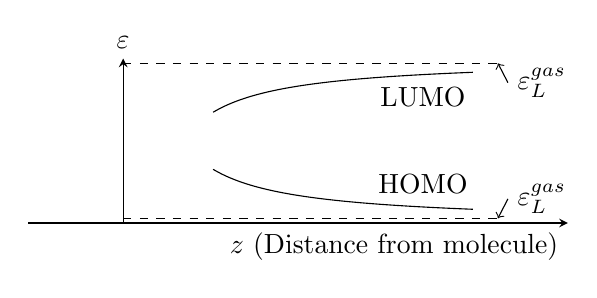
\begin{tikzpicture}
        \begin{axis}[
                axis lines=middle,
                ticks=none,
                y=35,
                xmin=-1,xmax=8,
                x label style={at={(current axis.right of origin)},anchor=north east},
                xlabel={$z$ (Distance from molecule)},
                y label style={anchor=south},
                ylabel={$\varepsilon$},
                domain=-10000:10000,
                restrict y to domain=-4:5,
                enlargelimits=true
                ]
            % parts:
            \addplot[black,domain=1.8:7,samples=102, unbounded coords=jump] {-1/(x)+2};
            \addplot[black,domain=1.8:7,samples=102, unbounded coords=jump] {+1/(x)+0.3};
            %\addplot[black,domain=2.001:10,samples=102, unbounded coords=jump] {1.7/(x-2)};
            %\addplot[black,domain=-3:10,samples=102] {(x-1)};
            \draw[dashed] (0,1.95) -- (7.5,1.95);
            \draw[<-] (7.5,1.95) -- (7.7,1.75) node[anchor=west] {$\varepsilon_L^{gas}$};
            \draw[dashed] (0,0.35) -- (7.5,0.35);
            \draw[<-] (7.5,0.35) -- (7.7,0.55) node[anchor=west] {$\varepsilon_L^{gas}$};
            %\draw (2,0.1) -- (2,-0.3) node[below] {$\omega_k$};
            \node at (6,1.6) {LUMO};
            \node at (6,0.7) {HOMO};
            %\node at (2.1,5) {$\Gamma(\omega)$};
            %\draw (2.9,1.89) circle (0.2);
            %\draw (0.1,-0.9) circle (0.2);
        \end{axis}
    \end{tikzpicture}
    \caption{Schematic illustration of the change in the ionisation potential (HOMO) and electron affinity (LUMO) when including screening from a nearby metal surface, calculated using the COH-SEX approximation with the classical screened potential (\eqref{eq:806}).}
    \label{fig:image_energies}
\end{figure}
\end{solution}